%%%%%%%%%%%%%%%%%%%%%%%%%%%%%%%%%%%%%%%%%
% Short Sectioned Assignment LaTeX Template Version 1.0 (5/5/12)
% This template has been downloaded from: http://www.LaTeXTemplates.com
% Original author:  Frits Wenneker (http://www.howtotex.com)
% License: CC BY-NC-SA 3.0 (http://creativecommons.org/licenses/by-nc-sa/3.0/)
%%%%%%%%%%%%%%%%%%%%%%%%%%%%%%%%%%%%%%%%%

%----------------------------------------------------------------------------------------
%	PACKAGES AND OTHER DOCUMENT CONFIGURATIONS
%----------------------------------------------------------------------------------------

\documentclass[paper=a4, fontsize=11pt]{scrartcl} % A4 paper and 11pt font size

% ---- Entrada y salida de texto -----

\usepackage[T1]{fontenc} % Use 8-bit encoding that has 256 glyphs
\usepackage[utf8]{inputenc}
%\usepackage{fourier} % Use the Adobe Utopia font for the document - comment this line to return to the LaTeX default

% ---- Idioma --------

\usepackage[spanish, es-tabla]{babel} % Selecciona el español para palabras introducidas automáticamente, p.ej. "septiembre" en la fecha y especifica que se use la palabra Tabla en vez de Cuadro

\usepackage{fancyhdr}

% ---- Otros paquetes ----

\usepackage{amsmath,amsfonts,amsthm} % Math packages
%\usepackage{graphics,graphicx, floatrow} %para incluir imágenes y notas en las imágenes
\usepackage{graphics,graphicx, float} %para incluir imágenes y colocarlas

% Para hacer tablas comlejas
%\usepackage{multirow}
%\usepackage{threeparttable}

%\usepackage{sectsty} % Allows customizing section commands
%\allsectionsfont{\centering \normalfont\scshape} % Make all sections centered, the default font and small caps

\usepackage{fancyhdr} % Custom headers and footers
\usepackage{url}
%\usepackage{hyperref}
\pagestyle{fancyplain} % Makes all pages in the document conform to the custom headers and footers
\fancyhead{} % No page header - if you want one, create it in the same way as the footers below
\fancyfoot[L]{} % Empty left footer
\fancyfoot[C]{} % Empty center footer
\fancyfoot[R]{\thepage} % Page numbering for right footer
\renewcommand{\headrulewidth}{0pt} % Remove header underlines
\renewcommand{\footrulewidth}{0pt} % Remove footer underlines
\setlength{\headheight}{13.6pt} % Customize the height of the header

\numberwithin{equation}{section} % Number equations within sections (i.e. 1.1, 1.2, 2.1, 2.2 instead of 1, 2, 3, 4)
\numberwithin{figure}{section} % Number figures within sections (i.e. 1.1, 1.2, 2.1, 2.2 instead of 1, 2, 3, 4)
\numberwithin{table}{section} % Number tables within sections (i.e. 1.1, 1.2, 2.1, 2.2 instead of 1, 2, 3, 4)

\setlength\parindent{0pt} % Removes all indentation from paragraphs - comment this line for an assignment with lots of text

\newcommand{\horrule}[1]{\rule{\linewidth}{#1}} % Create horizontal rule command with 1 argument of height

\usepackage{booktabs}




%----------------------------------------------------------------------------------------
%	TÍTULO Y DATOS DEL ALUMNO
%----------------------------------------------------------------------------------------

\title{	
\normalfont \normalsize 
\textsc{{\bf Metaheurísticas (2014-2015)} \\ Grado en Ingeniería Informática \\ Universidad de Granada} \\ [25pt] % Your university, school and/or department name(s)
\horrule{0.5pt} \\[0.4cm] % Thin top horizontal rule
\huge  Práctica 1 - Búsquedas por trayectorias simples \\ % The assignment title
\horrule{2pt} \\[0.5cm] % Thick bottom horizontal rule
}

\author{Ignacio Martín Requena} % Nombre y apellidos

\date{\normalsize\today} % Incluye la fecha actual

%----------------------------------------------------------------------------------------
% DOCUMENTO
%----------------------------------------------------------------------------------------
\usepackage{graphicx}
\usepackage{listings}
\usepackage{color}
\definecolor{gray97}{gray}{.97}
\definecolor{gray75}{gray}{.75}
\definecolor{gray45}{gray}{.45}
 

\lstset{ frame=Ltb,
     framerule=0pt,
     aboveskip=0.5cm,
     framextopmargin=3pt,
     framexbottommargin=3pt,
     framexleftmargin=0.4cm,
     framesep=0pt,
     rulesep=.4pt,
     backgroundcolor=\color{gray97},
     rulesepcolor=\color{black},
     %
     stringstyle=\ttfamily,
     showstringspaces = false,
     basicstyle=\small\ttfamily,
     commentstyle=\color{gray45},
     keywordstyle=\bfseries,
     %
     numbers=left,
     numbersep=15pt,
     numberstyle=\tiny,
     numberfirstline = false,
     breaklines=true,
   }
 


\lstdefinestyle{consola}
   {basicstyle=\scriptsize\bf\ttfamily,
    backgroundcolor=\color{gray75},
   }
 
\lstdefinestyle{C}
   {language=C,
   }



\begin{document}

\maketitle % Muestra el Título

\newpage %inserta un salto de página

\tableofcontents % para generar el índice de contenidos

\listoffigures

%\listoftables

\newpage




%----------------------------------------------------------------------------------------
%	Cuestion 1
%----------------------------------------------------------------------------------------
\section{Descripción del problema}
El problema de la asignación cuadrática (QAP) es un problema clásico en teoría de localización. En éste se trata de asignar N unidades a una cantidad N de sitios o localizaciones en donde se considera un costo asociado a cada una de las asignaciones. Este costo dependerá de las distancias y flujo entre unidades, además de un costo adicional por asignar cierta unidad a una localización específica. De este modo se buscará que este costo, en función de la distancia y flujo, sea mínimo.

Este problema tiene muchas aplicaciones, como el diseño de hospitales donde se pretende que los médicos recorran la menor distancia posible dependiendo de su especialidad, procesos de comunicaciones, diseño de teclados de un ordenador, diseño de circuitos eléctricos, diseño de terminarles en aeropuertos y, en general, todo aquel problema de optimización de trayectorias y localizaciones que posea un espacio de búsqueda considerablemente grande.

%----------------------------------------------------------------------------------------
%	Cuestion 2
%----------------------------------------------------------------------------------------
\section{Descripción de los algoritmos empleados}

En esta sección vamos a especificar las componentes comunes a todos los algoritmos empleados para la resolución del problema:

\begin{itemize}
	\item \textbf{Representación de la solución: }
	
	La forma más conveniente considerada para representar las soluciones es a través de las permutaciones de un conjunto. Esto quiere decir que si por ejemplo el problema tiene, por ejemplo, tamaño cuatro, una posible solución al problema sería N = \{1,4,2,3\}. De esta forma, si interpretamos los índices de este conjunto como las unidades, y el valor del índice como su localización, la localización 3 estaría asignada a la unidad 1, la 4 a la 2 y así sucesivamente.
	
	\item \textbf{Función objetivo:}
	
	Dado que el objetivo del problema es la minimización del costo total de todas las posibles soluciones, la función objetivo vendrá definida matemáticamente como:
	
	\begin{figure}[H]
		\centering
		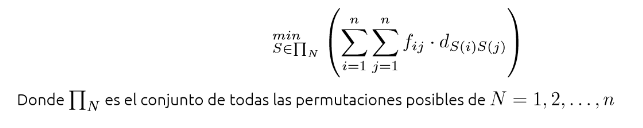
\includegraphics[scale=1.0]{Screenshot_2.png}
		\caption{Función objetivo}
		\label{}
	\end{figure}
	\newpage
	En forma de pseudicódigo nuestra función objetivo sería:
	
	\begin{lstlisting}[language=SH]
inicializamos el costo a 0
para cada fila de las matrices de distancia y flujo
	para cada posicion de las matrices de distancia y flujo
		costo += flujo[i][j] * distancia[[i]][sol[j]];

	\end{lstlisting}
	
	\item \textbf{Función factorizar:}
	
	Con el fin de aumentar la eficiencia y el tiempo de ejecución de nuestros algoritmos se implementa la función factorizar, que nos calcula la diferencia de costo entre una solución y otra, de esta forma evitamos el tener que calcular el costo de una solución de principio a fin.
	
	En forma de pseudicódigo nuestra función factorizar sería:
	
	\begin{lstlisting}[language=SH]
	
    inicializamos una variable suma a 0
    
    desde i=0 hasta N hacer
	    si i no coincide con ninguna de las localizaciones a inercambiar
		    realizar el coste del movimiento de intercambio como la sumatoria de la diferencia de todas las distancias nuevas menos las viejas multiplicadas por el flujo
	
	\end{lstlisting}
	\newpage
	\item \textbf{Función generar vecino:}	
	Esta función calcula una solución vecina a partir de una solución actual y dos posiciones a intercambiar.
	
	En forma de pseudicódigo nuestra función "swap" sería:
	
	\begin{lstlisting}[language=SH]

Crear un vector para guardar la nueva solucion
Para cada elemento de la solucion actual
	Copiar en el nuevo vector solucion
Guardar en una variable el valor de la posicion a intercambiar
Cambiar dicho valor por el contenido en la otra posicion
Asignar a la otra posicion el valor guardado en el paso 5 
Actualizar el costo de la solucion como el costo de la solucion inicial mas el factorizado
Devolver la nueva solucion

	\end{lstlisting}
	
		\item \textbf{Función generar solución aleatoria:}	
		Esta función calcula una solución inicial generada aleatoriamente.
		
		En forma de pseudicódigo nuestra función "getSolInicial" sería:
		
		\begin{lstlisting}[language=SH]
		
Creamos un vector de enteros con el tama\~{n}o de las matrices de flujo o distancia
Para cada posicion del vector creado
	Generamos un numero aleatorio compremndido entre la posicion actual y el tama\~{n}o del vector
	Introducimos este numero en el vector de soluciones iniciales
Calculamos el costo de la solucion inicial
Devolvemos la solucion y su costo
		\end{lstlisting}
\end{itemize} 


%----------------------------------------------------------------------------------------
%	Cuestion 3
%----------------------------------------------------------------------------------------
\section{Descripción del esquema de búsqueda y las operaciones de cada algoritmo}	
		
		\subsubsection{Búsqueda Local}
		Este algoritmo se compone de dos partes: La creación de la máscara Don't Look Bite y el propio algoritmo de búsqueda
		
		\begin{itemize}
			\item\textit{\textbf{ Don't Look Bite:}}
			Esta técnica permite focalizar la búsqueda en una zona del espacio en la que se puede encontrar una mejor solución. Con la máscara DLB vamos marcando con un 0 las zonas donde nos interesa explorar y con un 1 las que no. El 1 establece que se ha terminado una iteración del bucle interno sin escoger una solución.
			\newpage
			Una representación en pseudicódigo sería:
			
					\begin{lstlisting}[language=SH]
					
Inicializamos DLB a 0, y con un tamao igual que el del problema
Para i=1...n
	si DLB[i] == 0
		Para j=1...n
			vecino = intercambiar(i,j)
			comparar(vecino, solucion actual)
			si vecino mejor que solucion actual
				actual = vecino
			DLB[i] = DLB[j] = 0
					\end{lstlisting}
					
			\item \textbf{Búsqueda Local}
			Ahora mostramos una descripción en pseudocódigo del algoritmo que implementa la búsqueda local:
			
		\begin{lstlisting}[language=SH]
		
Declaramos una solucion que contendra la solucion vecina a la actual
Para cada i=0...n hacer
 Si DLB.at(i) == 0
  Generarvecino()
  Si costo vecino < costo actual
   solucion vecina = solucion actual
   DLB.at(i) = DLB.at(j) = 0
		Si solucion actual = solucion inicial
			DLB.at(i) = 1
Devolver solucion
	\end{lstlisting}
			
		\end{itemize}
		\subsubsection{Enfriamiento simulado}
		Para la metaheurística de enfriamiento simulado será necesario implementar dos algoritmos:
		
		\begin{itemize}
		
		\item \textbf{Función temperatura inicial}
		
		Esta función establece la temperatura inicial a partir de la siguiente fórmula:
		
			\begin{figure}[H]
				\centering
				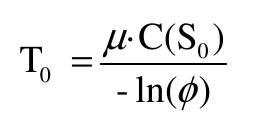
\includegraphics[scale=1.0]{Screenshot_3.png}
				\caption{Temperatura inicial}
				\label{}
			\end{figure}
			
		Donde T0 es la temperatura inicial, C(S0) es el coste de la solución inicial y $\phi\epsilon[0,1]$ es la probabilidad de aceptar una solución un $\mu$ por 1 peor que la inicial.	
		
		En forma de pseudocódigo nuestro algoritmo sería:	
		\begin{lstlisting}[language=SH]
Declaramos una variable de tipo real inicializada a 0 donde almacenaremos la temperatura inicial
Aplicamos la formula estipulada anteriormente
Devolvemos el resultado obtenido
		\end{lstlisting}
		
		\item \textbf{Algoritmo de enfriamiento simulado}
		Para la realización de este algoritmo tendremos una solución inicial generada aleatoriamente, una solución que será la mejor encontrada hasta el momento y una serie de parámetros que forman parte del algoritmo de enfriamiento simulado tales como la velocidad con la que enfriamos la temperatura (delta), las iteraciones realizadas, todo el espacio de vecindad de una solucion...
		
		El pseudocódigo del algoritmo que he implementado es el siguiente:
\begin{lstlisting}[language=SH]

Declaramos dos conjuntos de soluciones aleatorias
Inicializamos los parametros ro, delta, temperatura inicial, y demas contadores necesarios para controlar la parada del algoritmo
Mientras el numero de iteraciones < n*10 o T < 0.001
	Declaramos dos contadores para controlar el descenso de la temperatura
	Mientras ambos contadores sean menores que un valor inicial establecido
		GenerarVecindario
		Para cada i=1..n y siempre que i < n*(n-1)/2
			Seleccionamos un vecino
			Calculamos la diferencia de coste entre la solucion y el vecino generado
			Definimos la variable de probabilidad de incremento energetico e
			Si la diferencia es menor que 0 o un numero aleatorio es menor que e
				Guardamos la solucion en una variable
				Si esta solucion es mejor que la declarada inicialmente
					Se elige como mejor solucion
					Se pone el numero de iteraciones a 0
	Actualizamos la temperatura, las iteraciones y el valorestablecido para los contadores
Devolvemos la solucion mejor

\end{lstlisting}
		
		\end{itemize}	
		\subsubsection{Búsqueda tabú}
	
Para la búsqueda tabú en primer lugar debo comentar que me ha sido imposible hacer una implementación buena con multiarranque, por lo que he optado por realizar unn algoritmo de busqueda tabú del mejor de todo los vecinos. 

El algoritmo en pseudocódigo es el siguiente:

\begin{lstlisting}[language=SH]

Declaramos e inicializamos como correspondados contadores, una lista tabu, una variable para almacenar las vecindades, una variable para almacenar la mejor solucion y un conjunto de soluciones para almacenar la actual
Inicializamos a NULL cada un de los componentes de la lista tabu
Mientras i < dim*10
	Obtenemos todos los vecinos a partir del actual
	Colocamos un costo muy alto a los estados que se encuentran en la lista Tabu comprobando si un estado del vecindario y otro de la lista tabu son iguales
	Buscamos la mejor solucion de la vecindad que no este en lTabu
	Si costo actual menor que costo anterior
		Copiar solucion actual como mejor solucion y costo actual como mejor costo
		Poner el contador i a 0
	Incrementar contadores
Devolver solucion
\end{lstlisting}

Esta implementación de la búsqueda tabú se basa unicamente en la intensificación, dado que se vuelve a la mejor solución obtenida hasta el momento y se continua a partir de ella. La ausencia de diversificación puede hacer que caigamos en óptimos locales muy fácilmente, por lo que es probable que los resultados de esta implementación no sean del todo buenos.
%----------------------------------------------------------------------------------------
%	Cuestion 4
%----------------------------------------------------------------------------------------
\newpage
\section{Algoritmo de comparación: Greedy}
Este algoritmo no hace mas que calcular los potenciales de cada unidad y de cada localización, los ordena y asigna el de mayor flujo al de menor distancia.

En pseudocódigo sería algo como:

\begin{lstlisting}[language=SH]
Declaramos un estado solucion
Ordenamos por flujo la matriz de flujo y por distancia la de distancia
Para i=0..n
	Asignamos al elemento determinado por flujo del estado solucion el elemento distancia (podemos hacerlo asi ya que hemos ordenado los vectores previamente.)
Asignamos el costo de la solucion
Devolvemos el estado

\end{lstlisting}

%----------------------------------------------------------------------------------------
%	Cuestion 5
%----------------------------------------------------------------------------------------
\section{Procedimiento considerado para desarrollar la práctica}
Para la realización de esta práctica me he basado en una implementación que he encontrado por internet\footnote{\url{http://quadratic-assignation.googlecode.com/svn-history/r44/trunk/qap.cpp}} dado que me ha resultado facil de entender y elegante, sobre todo por la utilización del struc de Estados. Aun así la modificación a este codigo ha sido casi entera, sobre todo en la forma de leer el archivo dat, el algoritmo de busqueda local, de enfriamiento y el tabu. Me ha resultado de gran ayuda ya que tenía algunos operadores de copia implementados. El resto de ayudas han venido sobre todo de mano de los apuntes de clase, del guion de prácticas o de charlas con compañeros de clase.

%----------------------------------------------------------------------------------------
%	Cuestion 6
%----------------------------------------------------------------------------------------
\section{Experimentos y análisis de los resultados}

Los problemas que he empelado han sido los mismos que los que vienen en la plantilla que se nos proporciona. Para cada caso, los parámetros para su ejecución son:

./qap <Metaheuristica> <archivo de entrada> <semilla>\\

donde metaheurística indica la metaheurística a usar:\\
1) Greedy\\
2) Busqueda Local\\
3) Enfriamiento Simulado\\
4) Busqueda Tabú\\

La semilla usada ha sido la \textbf{28345234} 

A continuación se muestran las tablas con los resultados obtenidos:

	\begin{figure}[H]
		\centering
		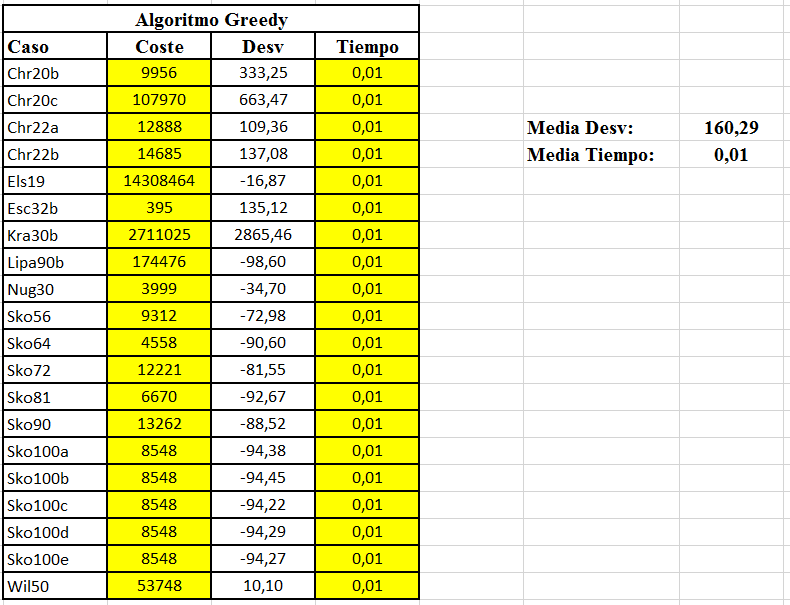
\includegraphics[scale=1.0]{Screenshot_4.png}
		\caption{Resultados Greedy}
		\label{}
	\end{figure}

	\begin{figure}[H]
		\centering
		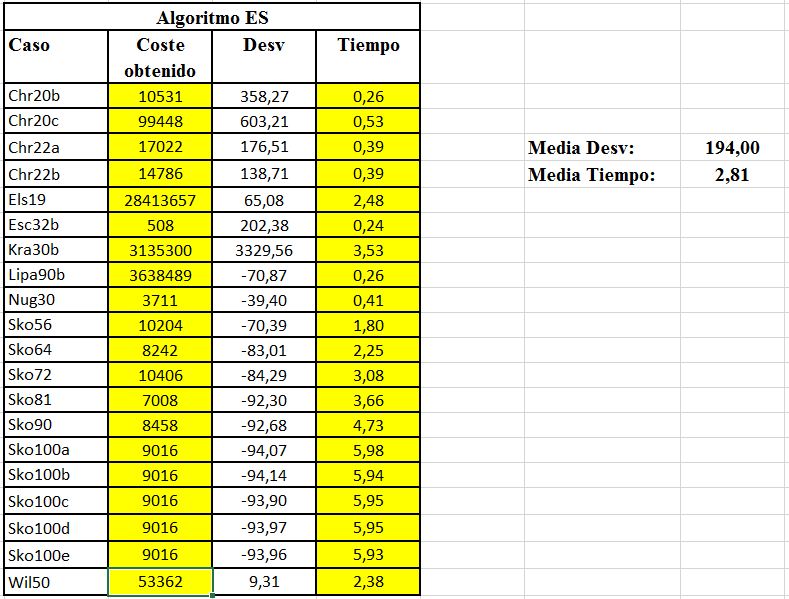
\includegraphics[scale=1.0]{Screenshot_5.png}
		\caption{Resultados Busqueda local}
		\label{}
	\end{figure}

	\begin{figure}[H]
		\centering
		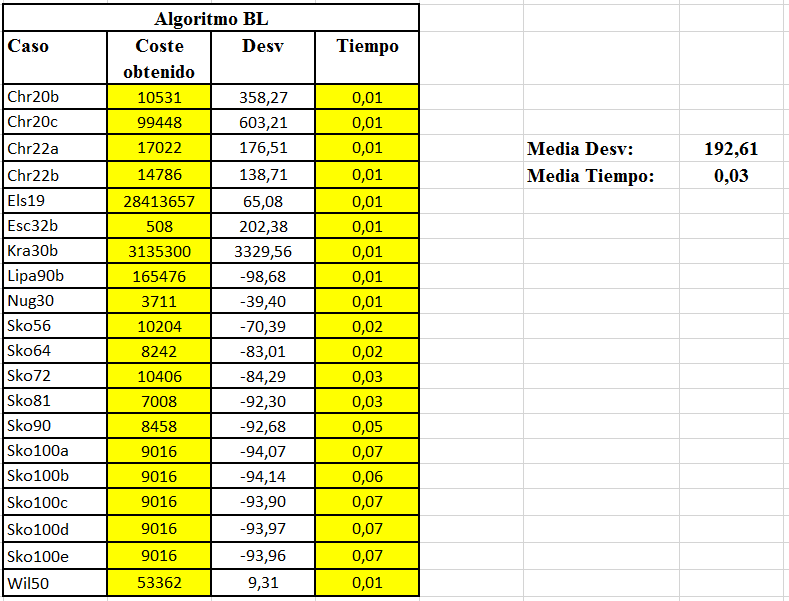
\includegraphics[scale=1.0]{Screenshot_1.png}
		\caption{Resultados enfriamiento simulado}
		\label{}
	\end{figure}

	\begin{figure}[H]
		\centering
		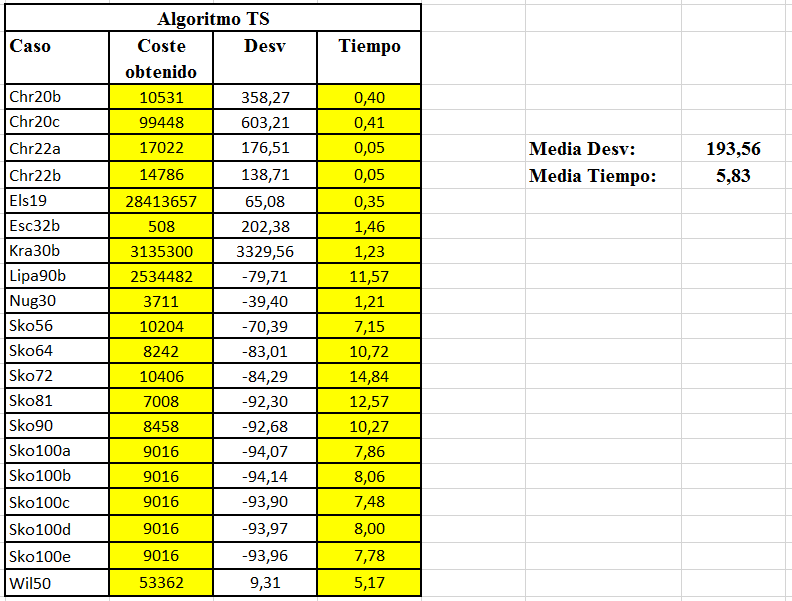
\includegraphics[scale=1.0]{Screenshot_6.png}
		\caption{Resultados búsqueda tabú}
		\label{}
	\end{figure}

Como se puede observar, estos algoritmos son muy útiles para problemas de gran tamaño, donde la capacidad de cómputo y la forma en que se realizan las búsquedas son cruciales. Aun así, podemos ver que aunque la busqueda tabú obtiene resultados considerablemente buenos para espacios de busqueda grandes, quizá hubiera sido necesaria algún tipo de reinicialización tal y como se sugería en la practica para aprovechar al máximo su potencial.

\end{document}